\newpage
\section{Durchführung}
\label{sec:Durchführung}

Der Aufbau zur Ermittlung der Suszeptibilität beinhaltet einen Sinusgenerator, eine Brückenschaltung mit Spule und den Proben, einen Selektivverstärker und ein AC Millivoltmeter.
Die \autoref{fig:aufbau} zeigt den Aufbau.

\begin{figure}[htbp]
    \centering
    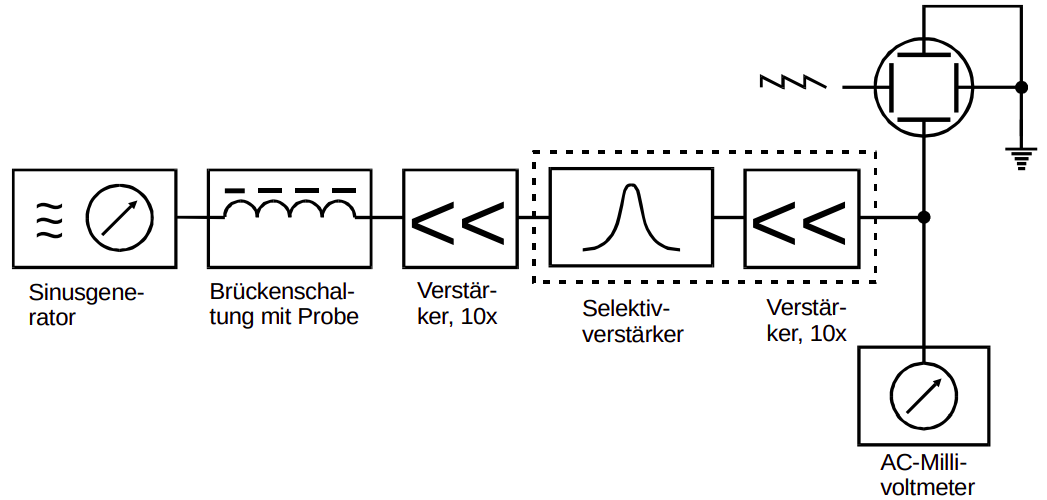
\includegraphics[scale=0.3]{Data/Aufbau.png}
    \caption{Dies ist der Aufbau des Versuchs zur Ermittlung der Suszeptibilität von seltenen Erden.}
    \label{fig:aufbau}
\end{figure}

Zunächst wird auf dem Sinusgenerator eine Speisespannung generiert, die in die Brückenschaltung geleitet wird.
Hierbei wird eine Spannung gesucht, die bei ca. $\SI{35}{\kilo\hertz}$ liegt und beim Millivoltmeter einen maximalen Ausschlag anzeigt.
Ist diese Spannung gefunden, wird das Minimum der Brückenspannung mittels des verstellbaren Widerstands auf der Brückenschaltung ermittelt und zusammen mit dem Widerstand notiert.
Wenn eine Probe in die Spule gelegt wird, muss dies ebenfalls gemacht werden.\\
Für drei Proben soll so je drei Mal die Brückenspannung mit und ohne Probe ermittelt werden.